
\indent \indent
After optimization of the variables during cross validation phase of the experiment, the network is retrained using all the available signals using the same setup as in cross validation phase.  The remaining portion of the signals excluding the data for last 31 days is used to make the extended system states. These extended system states and the computed $\mathbf{W}^{out}$ is used to make the prediction using Equation \eqref{eq:prediction}. \\
There are 31 output neurons, each of which makes the prediction for $n=1\hdots,31$ days ahead. The network optimized during cross validation phase and retrained afterward is used to predict the number of views for the month of December 2016. The error for each prediction horizons is calculated as NRMSE. The testing error measures for each prediction horizons are plotted in Figure \ref{fig:nrmsevspw}. The predicted number of views and the actual number of views for different prediction horizons, are plotted in Figure \ref{fig:realvspredicted}. As seen in Figure \ref{fig:nrmsevspw}, usually the NRMSE for the shorter prediction horizon is smaller and for the longer prediction horizon is bigger. The NRMSE values do not increase linearly with the prediction horizon. One of the reasons for this could be, I assume, that some of the features like the biweekly or triweekly repetition of some pattern in the data might be stronger than other frequencies. For example: the page might have received proportional views at the end of every two weeks.
\\
The values for the optimized parameters that worked best for this experiment are presented in Table \textcolor{blue}{2}. Also, the mean training error and testing error for all 31 prediction horizons are given in Table \textcolor{blue}{3}.\\


\begin{center}
		\label{table:error}
		
 \begin{tabular}{|c|c|} \hline

     & value \\ \hline
	 Mean training NRMSE & 1.02\\ \hline
	 Mean Testing NRMSE & 1.04 \\ \hline

\end{tabular}
\captionof{table}{Mean training and testing errors of all 31 prediction horizons.  }
\end{center}
% \vspace{1cm}
\begin{center}
\begin{tabular}{|c|c|c|} \hline
	 \multicolumn{2}{|l|}{ Parameters }& Optimized value\\ \hline
	 \multicolumn{2}{|l|}{ $sf^{\mathbf{W}}$}& 0.9\\ \hline
	 \multicolumn{2}{|l|}{$sf^{\mathbf{Win}}$}& 0.3 \\ \hline
	 \multicolumn{2}{|l|}{$sf^{\mathbf{B}}$}& 0.001\\ \hline
	 \multicolumn{2}{|l|}{$\beta$}& 0.95\\ \hline
	 \multicolumn{2}{|l|}{$sf_{sine}$} & 0.8\\ \hline
	 \multicolumn{2}{|l|}{ $sf_{add}$} &  0.6\\ \hline
	 \multirow{3}{*}{$\alpha$} & FAST & 0.1\\ \cline{2-3}
	                   & MEDIUM &0.5\\ \cline{2-3}
					   & SLOW &  0.9 \\\hline	
\end{tabular}
\captionof{table}{Optimized values for control parameters} \label{table:optimized} 
\end{center}

	
  \begin{figure}[h]
     \centering
     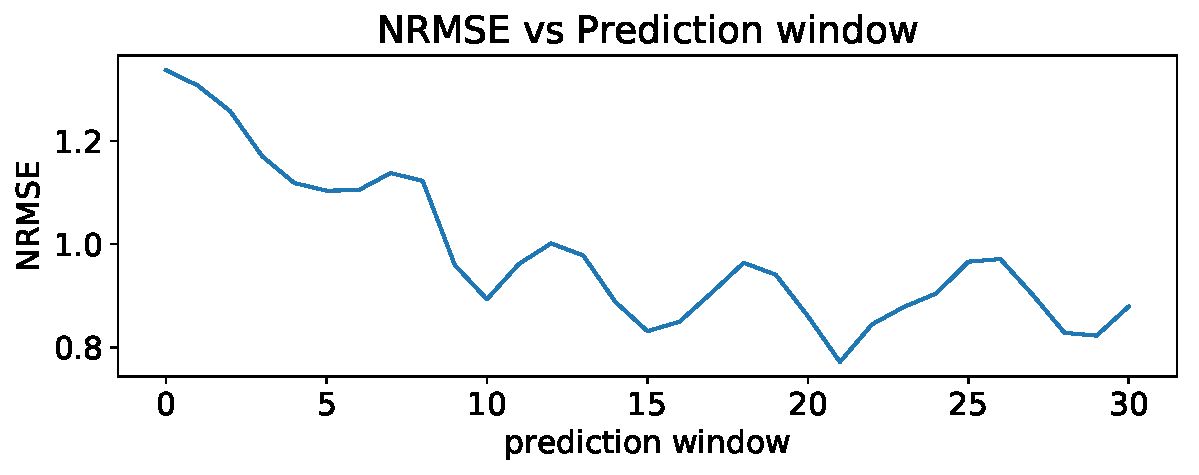
\includegraphics[width=\textwidth]{./results/images/nrmsevspwrec}
	 \label{fig:nrmsevspredicted}
      \caption{NRMSE for different prediction window ranges}\label{fig:nrmsevspw}
  \end{figure}
 
  \begin{figure}[]
      \begin{subfigure}[h]{1\textwidth}
          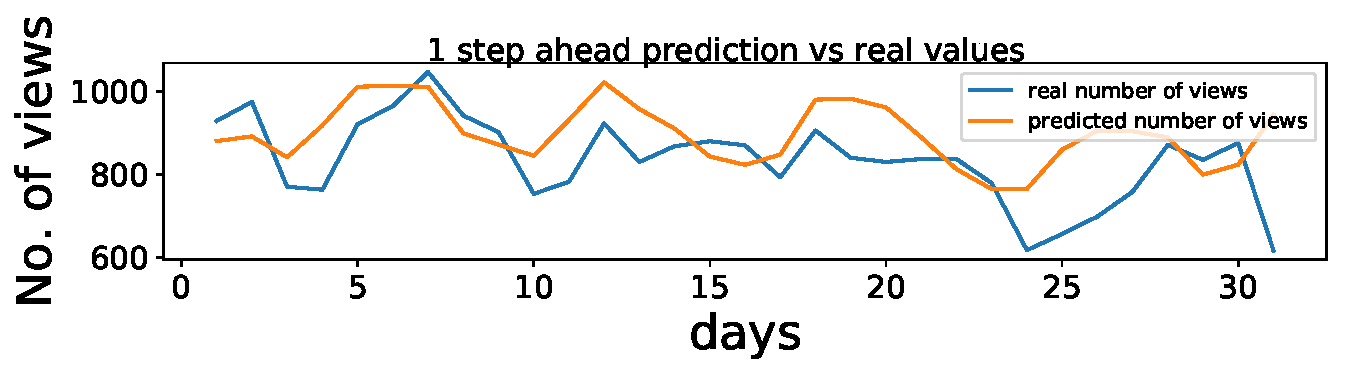
\includegraphics[width=\textwidth]{./results/images/1stepAhead}
      \end{subfigure}
	  
      \begin{subfigure}[h]{1\textwidth}
          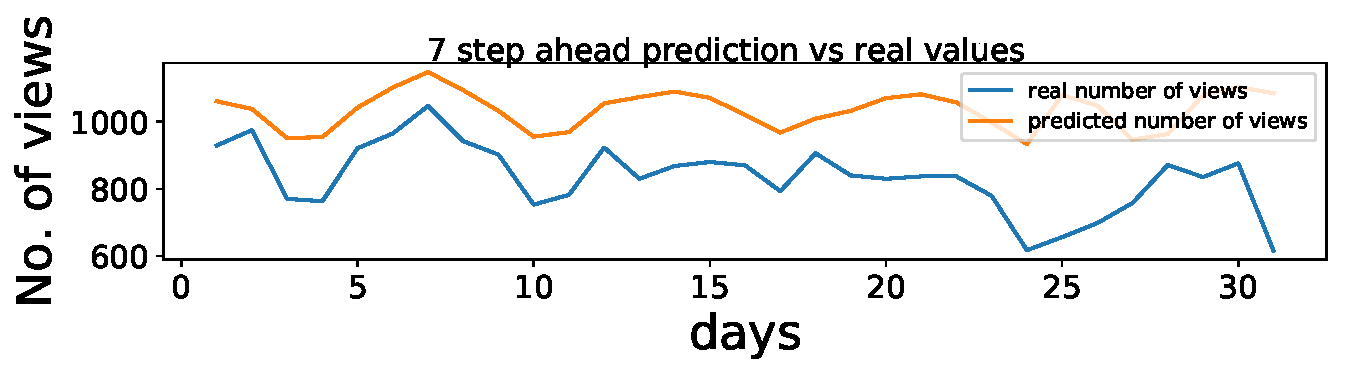
\includegraphics[width=\textwidth]{./results/images/7stepAhead}
      \end{subfigure}
	  
      \begin{subfigure}[h]{1\textwidth}
          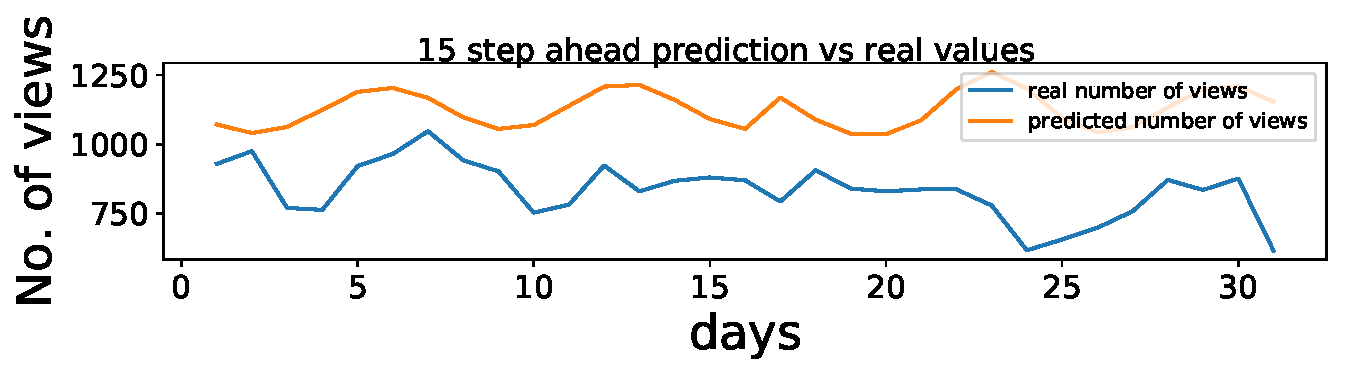
\includegraphics[width=\textwidth]{./results/images/15stepAhead}
      \end{subfigure}
	  
      \begin{subfigure}[h]{1\textwidth}
          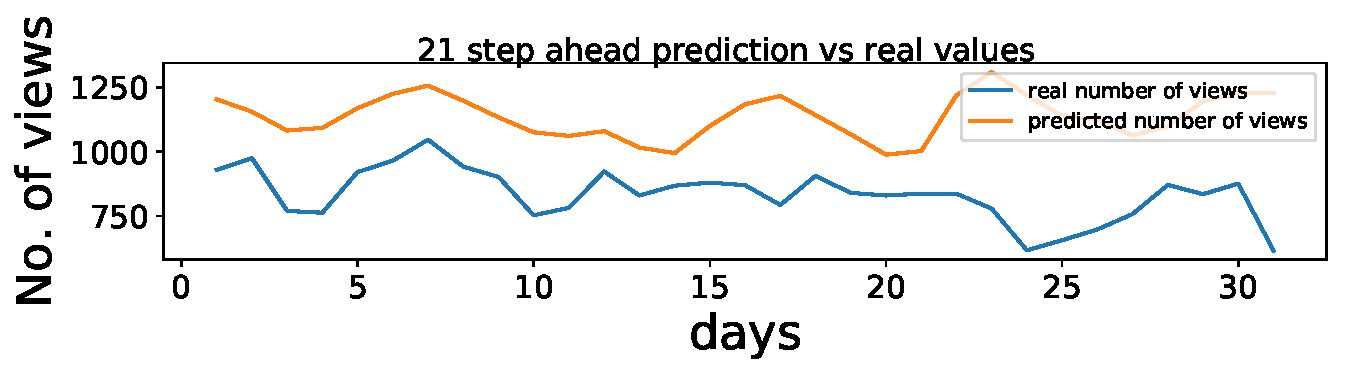
\includegraphics[width=\textwidth]{./results/images/21stepAhead}
      \end{subfigure}
	  
      \begin{subfigure}[h]{1\textwidth}
          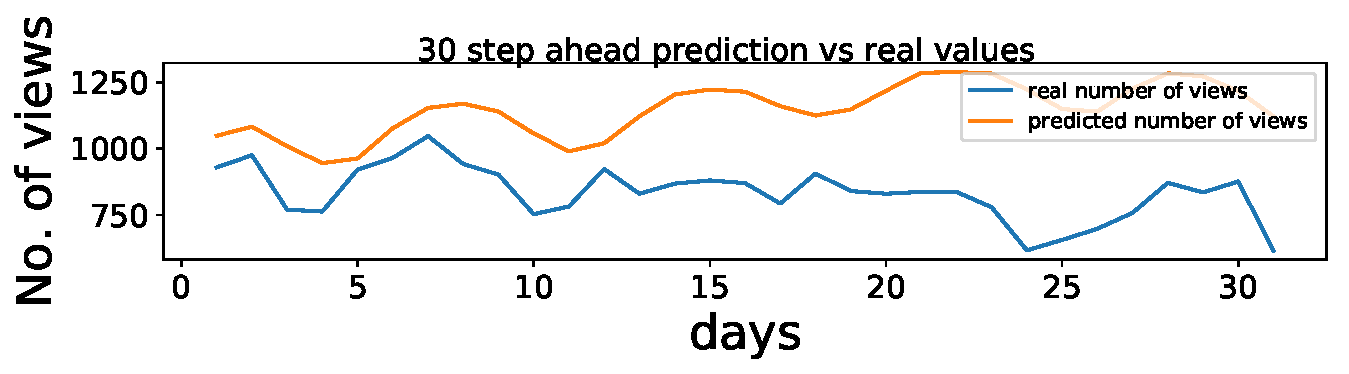
\includegraphics[width=\textwidth]{./results/images/30stepAhead}
      \end{subfigure}
	 
      \caption{Real values vs predicted values for different prediction horizons }\label{fig:realvspredicted}
  \end{figure}
  
 
 % \begin{figure}[h]
 %    \centering
 %    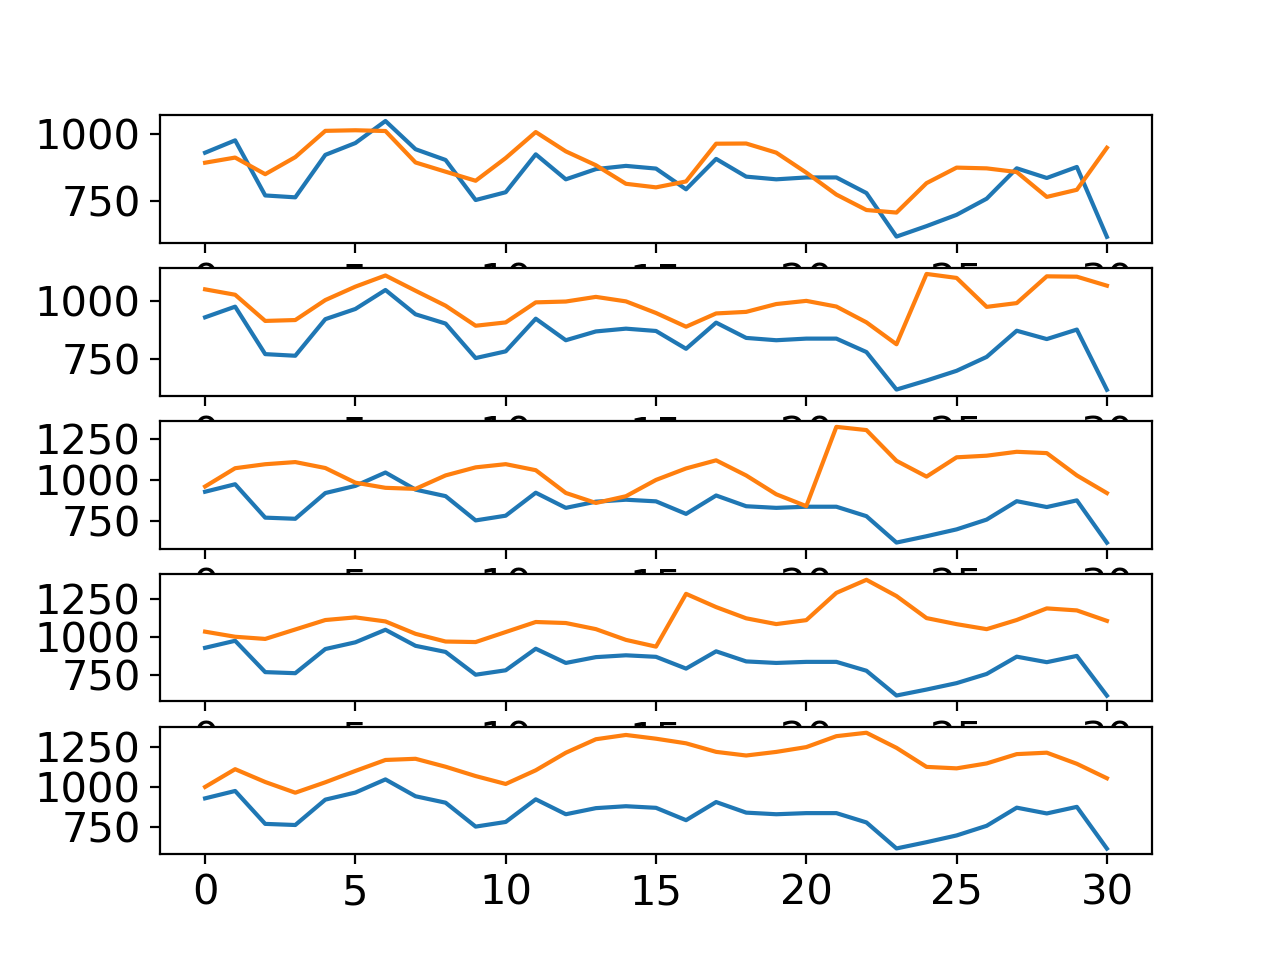
\includegraphics[width=\textwidth]{./results/images/realvspredicted}
 %
 %     \caption{NRMSE for different prediction window ranges}\label{fig:realvspredicted}
 % \end{figure}
 
 


 \subsection*{Observation}
 During the process of tuning the parameters of the network, it was observed that data preprocessing affects the prediction by the network at a higher extent compared other factors. The reason for it, I believe, is that the preprocessing steps scale down the outliers in the training signal and also scale up the previously hidden features in the signal. Adding an additional sine wave to the input signal also significantly improves the prediction (NRMSE decreases in the order of $0.1$).  This is because a sine wave signal of period $7$  gives the insight of weeks to the network. Therefore, on adding an extra sine wave signal as the input, causes the network to easily identify any weekly pattern present in the main input signal. However, adding other additional inputs do not have a significant impact on the prediction (NRMSE decreases in the order of $0.01$). This could be because these additional signals are highly correlated to the main input signal and thus do not add much additional information to the network. During cross validation phase, with the smaller values of regularization coefficient, $\beta$ it was observed that the predicted values in some of the folds deviated highly from the real values as well as the mean value. This is because with a very small regularization coefficient, the output weights get bigger and thus, even a small perturbation in the input signal can lead to a strong perturbation in the predicted signal. Best results were obtained by the network when the scaling factors for $sf_W$ and $sf_{Win}$ were in the range of $0.5 - 1.5$ and $0.3 - 0.6$ despite the fact that the difference in the performance was barely noticeable with any values assigned in that range. 
 
 
 